% --- Slide 11 ---
\begin{frame}{Tổng quan pipeline render}
    \begin{itemize}
        \item World $\to$ Camera: biến đổi hệ toạ độ bằng view transform $(R, t)$
        \item Projection: chiếu các Gaussian 3D xuống mặt phẳng ảnh 2D
        \item Tiling: xác định tile ảnh nào chịu ảnh hưởng bởi mỗi Gaussian
        \item Sorting: sắp xếp Gaussian theo độ sâu (depth) trong từng tile
        \item Alpha blending tuần tự $\to$ màu pixel cuối cùng
    \end{itemize}
    \vspace{0.3cm}
    \centering
    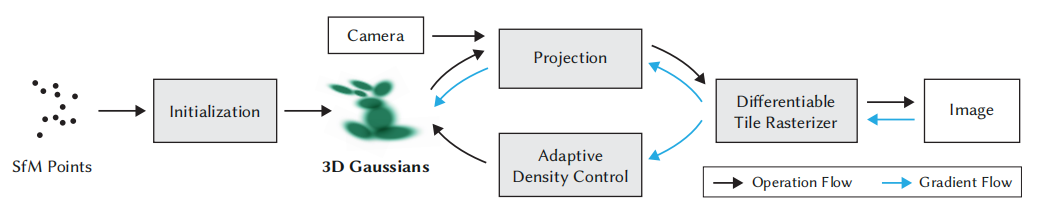
\includegraphics[width=0.95\linewidth]{pipe.png}
    \captionof{figure}{Pipeline render 3D Gaussian Splatting}
\end{frame}

% --- Slide 12 ---
\begin{frame}{Chiếu camera pinhole}
    \begin{columns}
        \begin{column}{0.48\textwidth}
            \begin{itemize}
                \item World $\to$ Camera: nhân với ma trận quay $R$ và tịnh tiến $t$
                \item Chiếu phối cảnh theo mô hình pinhole với tiêu cự $f$ và điểm chính (principal point)
                \item Công thức chiếu cơ bản:
                \[
                    x' = f\frac{x}{z}, \qquad y' = f\frac{y}{z}
                \]
                \item Kết quả: toạ độ tâm Gaussian trên ảnh 2D
            \end{itemize}
        \end{column}
        \begin{column}{0.48\textwidth}
            \centering
            
\includegraphics[width=0.95\linewidth]{ch3_pinhole_projection.png}
            \captionof{figure}{Mô hình chiếu pinhole}
        \end{column}
    \end{columns}
\end{frame}

% --- Slide 13 ---
\begin{frame}{Chiếu hiệp phương sai (EWA splatting)}
    \begin{itemize}
        \item Phép chiếu phối cảnh phi tuyến $\to$ xấp xỉ tuyến tính cục bộ bằng Jacobian $J$ tại tâm Gaussian
        \item Hiệp phương sai 2D sau chiếu:
        \[
            \Sigma' = J\,W\,\Sigma\,W^{T}J^{T}
        \]
        trong đó $W$ là phần quay của view matrix
        \item Kết quả: một ellipse 2D trên ảnh cho mỗi Gaussian 3D
        \item Kỹ thuật này gọi là \textbf{Elliptical Weighted Average (EWA) splatting}
    \end{itemize}
    \vspace{0.2cm}
    \centering
    
\includegraphics[width=0.6\linewidth]{ch3_ewa_projection.png}
    \captionof{figure}{Chiếu hiệp phương sai theo EWA splatting}
\end{frame}

% --- Slide 14 ---
\begin{frame}{Compact Box -- đòn bẩy tăng tốc \#1 của FastGS}
\begin{columns}[T]
\begin{column}{0.52\textwidth}
\footnotesize
    \begin{itemize}
        \item Mặc định: bounding-box $3\sigma$ -- khá rộng, chạm nhiều tile không cần thiết
        \item FastGS thay bằng \textbf{compact box}: vùng ảnh hưởng 2D nhỏ hơn, điều chỉnh bằng hệ số \texttt{-{}-mult}
        \item Mặc định \texttt{mult = 0.5}; tăng lên \texttt{0.7} cho cảnh lớn/phức tạp
        \item Kết quả: giảm đáng kể số tile mỗi Gaussian phải rasterize
    \end{itemize}
\end{column}
\begin{column}{0.48\textwidth}
    \centering
    
\includegraphics[width=0.95\linewidth]{ch3_compact_box.png}
    \captionof{figure}{\footnotesize So sánh bounding-box mặc định và compact box}
\end{column}
\end{columns}
\end{frame}

% --- Slide 15 ---
\begin{frame}{Tỉ lệ diện tích ảnh hưởng tile}
\begin{columns}[T]
\begin{column}{0.5\textwidth}
\footnotesize
    \begin{itemize}
        \item Số tile bị một Gaussian "chạm" tỉ lệ thuận với diện tích ellipse chiếu của nó trên ảnh
        \item Compact box giúp giảm tỉ lệ diện tích này mà không làm giảm chất lượng render đáng kể
        \item Đây là cơ sở lý thuyết cho việc tăng tốc rasterization của FastGS
    \end{itemize}
\end{column}
\begin{column}{0.5\textwidth}
    \centering
    
\includegraphics[width=0.95\linewidth]{ch3_area_ratio.png}
    \captionof{figure}{\footnotesize Tỉ lệ diện tích ảnh hưởng khi thay đổi compact box}
\end{column}
\end{columns}
\end{frame}

% --- Slide 16 ---
\begin{frame}{Rasterizer khả vi theo tile (CUDA)}
    \begin{itemize}
        \item Ảnh được chia thành lưới tile (ví dụ $16 \times 16$ pixel)
        \item Mỗi tile lưu danh sách các Gaussian chạm tới nó
        \item Danh sách này được sort theo độ sâu (depth) trước khi blend
        \item Xử lý song song trên GPU: mỗi thread-block CUDA đảm nhận một tile
        \item Cài đặt trong module \texttt{submodules/diff-gaussian-rasterization\_fastgs/}
        \item Toàn bộ quá trình khả vi $\to$ hỗ trợ lan truyền ngược gradient
    \end{itemize}
\end{frame}

% --- Slide 17 ---
\begin{frame}{Trường alpha (opacity field)}
\begin{columns}[T]
\begin{column}{0.52\textwidth}
\footnotesize
    \begin{itemize}
        \item Mỗi Gaussian 2D đã chiếu tạo ra một trường độ mờ liên tục trên ảnh
        \item Công thức trường alpha:
        \[
            \alpha(p) = \alpha_i \cdot G'_i(p)
        \]
        \item $G'_i$ là hàm Gaussian 2D chuẩn hoá theo hiệp phương sai $\Sigma'$
        \item Giá trị $\alpha(p)$ càng lớn khi $p$ càng gần tâm ellipse
    \end{itemize}
\end{column}
\begin{column}{0.48\textwidth}
    \centering
    
\includegraphics[width=0.85\linewidth]{ch4_alpha_field.png}
    \captionof{figure}{\footnotesize Trường alpha của một Gaussian 2D}
\end{column}
\end{columns}
\end{frame}

% --- Slide 18 ---
\begin{frame}{Alpha blending (front-to-back)}
    \begin{itemize}
        \item Màu pixel là tổng có trọng số của các Gaussian chồng nhau theo thứ tự độ sâu
        \item Công thức blend:
        \[
            C = \sum_i c_i\,\alpha_i\,T_i, \qquad T_i = \prod_{j<i}(1-\alpha_j)
        \]
        \item $T_i$: độ truyền sáng còn lại (transmittance) trước Gaussian thứ $i$
        \item Gaussian gần camera hơn đóng góp trọng số lớn hơn
    \end{itemize}
    \vspace{0.2cm}
    \centering
    
\includegraphics[width=0.55\linewidth]{ch4_alpha_blend_stack.png}
    \captionof{figure}{Chồng lớp alpha blending theo độ sâu}
\end{frame}

% --- Slide 19 ---
\begin{frame}{Suy giảm độ truyền sáng (transmittance decay)}
\begin{columns}[T]
\begin{column}{0.52\textwidth}
\footnotesize
    \begin{itemize}
        \item $T_i$ giảm dần theo cấp số nhân khi càng nhiều Gaussian che phía trước
        \item Khi $T_i \approx 0$: các Gaussian phía sau gần như không đóng góp vào màu pixel
        \item Cho phép \textbf{early stopping}: dừng xử lý sớm để tối ưu tốc độ render
        \item Đây là một trong các kỹ thuật tăng tốc quan trọng của rasterizer
    \end{itemize}
\end{column}
\begin{column}{0.48\textwidth}
    \centering
    
\includegraphics[width=0.9\linewidth]{ch4_transmittance_decay.png}
    \captionof{figure}{\footnotesize Suy giảm transmittance theo số lớp Gaussian}
\end{column}
\end{columns}
\end{frame}

% --- Slide 20 ---
\begin{frame}{Tổng kết phương trình render}
    \begin{itemize}
        \item Phương trình render đầy đủ:
        \[
            C(p) = \sum_i c_i\,\alpha_i \prod_{j<i}(1-\alpha_j)
        \]
        \item Khả vi theo mọi tham số: vị trí $\mu$, hiệp phương sai $\Sigma$, độ mờ $\alpha$, hệ số SH
        \item Cho phép huấn luyện trực tiếp bằng gradient descent từ ảnh RGB quan sát được
    \end{itemize}
    \vspace{0.4cm}
    \centering
    \begin{tikzpicture}[node distance=1.1cm, every node/.style={font=\footnotesize}]
        \node (g3d) {Gaussian 3D};
        \node (proj) [right=of g3d] {Chiếu 2D};
        \node (alpha) [right=of proj] {Trường alpha};
        \node (blend) [right=of alpha] {Blend};
        \node (pixel) [right=of blend] {Pixel};
        \draw[-Latex] (g3d) -- (proj);
        \draw[-Latex] (proj) -- (alpha);
        \draw[-Latex] (alpha) -- (blend);
        \draw[-Latex] (blend) -- (pixel);
    \end{tikzpicture}
\end{frame}
